%%%%%%%%%%%%%%%%%%%%%%%%%%%%%%%%%%%%%%%%%
% Cleese Assignment (For Students)
% LaTeX Template
% Version 2.0 (27/5/2018)
%
% This template originates from:
% http://www.LaTeXTemplates.com
%
% Author:
% Vel (vel@LaTeXTemplates.com)
%
% License:
% CC BY-NC-SA 3.0 (http://creativecommons.org/licenses/by-nc-sa/3.0/)
% 
%%%%%%%%%%%%%%%%%%%%%%%%%%%%%%%%%%%%%%%%%

%----------------------------------------------------------------------------------------
%	PACKAGES AND OTHER DOCUMENT CONFIGURATIONS
%----------------------------------------------------------------------------------------

\documentclass[11pt]{article}

%%%%%%%%%%%%%%%%%%%%%%%%%%%%%%%%%%%%%%%%%
% Cleese Assignment
% Structure Specification File
% Version 1.0 (27/5/2018)
%
% This template originates from:
% http://www.LaTeXTemplates.com
%
% Author:
% Vel (vel@LaTeXTemplates.com)
%
% License:
% CC BY-NC-SA 3.0 (http://creativecommons.org/licenses/by-nc-sa/3.0/)
% 
%%%%%%%%%%%%%%%%%%%%%%%%%%%%%%%%%%%%%%%%%

%----------------------------------------------------------------------------------------
%	PACKAGES AND OTHER DOCUMENT CONFIGURATIONS
%----------------------------------------------------------------------------------------

\usepackage{lastpage} % Required to determine the last page number for the footer

\usepackage{graphicx} % Required to insert images

\setlength\parindent{0pt} % Removes all indentation from paragraphs

\usepackage[most]{tcolorbox} % Required for boxes that split across pages

\usepackage{booktabs} % Required for better horizontal rules in tables

\usepackage{listings} % Required for insertion of code

\usepackage{etoolbox} % Required for if statements


%----------------------------------------------------------------------------------------
%	MARGINS
%----------------------------------------------------------------------------------------

\usepackage{geometry} % Required for adjusting page dimensions and margins

\geometry{
	paper=a4paper, % Change to letterpaper for US letter
	top=3cm, % Top margin
	bottom=3cm, % Bottom margin
	left=2.5cm, % Left margin
	right=2.5cm, % Right margin
	headheight=14pt, % Header height
	footskip=1.4cm, % Space from the bottom margin to the baseline of the footer
	headsep=1.2cm, % Space from the top margin to the baseline of the header
	%showframe, % Uncomment to show how the type block is set on the page
}

%----------------------------------------------------------------------------------------
%	FONT
%----------------------------------------------------------------------------------------

\usepackage[utf8]{inputenc} % Required for inputting international characters
\usepackage[T1]{fontenc} % Output font encoding for international characters

\usepackage[sfdefault,light]{roboto} % Use the Roboto font

%----------------------------------------------------------------------------------------
%	HEADERS AND FOOTERS
%----------------------------------------------------------------------------------------

\usepackage{fancyhdr} % Required for customising headers and footers

\pagestyle{fancy} % Enable custom headers and footers

\lhead{\small\assignmentClass\ifdef{\assignmentClassInstructor}{\ (\assignmentClassInstructor):}{}\ \assignmentTitle} % Left header; output the instructor in brackets if one was set
\chead{} % Centre header
\rhead{\small\ifdef{\assignmentAuthorName}{\assignmentAuthorName}{\ifdef{\assignmentDueDate}{Due\ \assignmentDueDate}{}}} % Right header; output the author name if one was set, otherwise the due date if that was set

\lfoot{} % Left footer
\cfoot{\small Page\ \thepage\ of\ \pageref{LastPage}} % Centre footer
\rfoot{} % Right footer

\renewcommand\headrulewidth{0.5pt} % Thickness of the header rule

%----------------------------------------------------------------------------------------
%	MODIFY SECTION STYLES
%----------------------------------------------------------------------------------------

\usepackage{titlesec} % Required for modifying sections

%------------------------------------------------
% Section

\titleformat
{\section} % Section type being modified
[block] % Shape type, can be: hang, block, display, runin, leftmargin, rightmargin, drop, wrap, frame
{\Large\bfseries} % Format of the whole section
{\assignmentQuestionName~\thesection} % Format of the section label
{6pt} % Space between the title and label
{} % Code before the label

\titlespacing{\section}{0pt}{0.5\baselineskip}{0.5\baselineskip} % Spacing around section titles, the order is: left, before and after

%------------------------------------------------
% Subsection

\titleformat
{\subsection} % Section type being modified
[block] % Shape type, can be: hang, block, display, runin, leftmargin, rightmargin, drop, wrap, frame
{\itshape} % Format of the whole section
{(\alph{subsection})} % Format of the section label
{4pt} % Space between the title and label
{} % Code before the label

\titlespacing{\subsection}{0pt}{0.5\baselineskip}{0.5\baselineskip} % Spacing around section titles, the order is: left, before and after

\renewcommand\thesubsection{(\alph{subsection})}

%----------------------------------------------------------------------------------------
%	CUSTOM QUESTION COMMANDS/ENVIRONMENTS
%----------------------------------------------------------------------------------------

% Environment to be used for each question in the assignment
\newenvironment{question}{
	\vspace{0.5\baselineskip} % Whitespace before the question
	\section{} % Blank section title (e.g. just Question 2)
	\lfoot{\small\itshape\assignmentQuestionName~\thesection~continued on next page\ldots} % Set the left footer to state the question continues on the next page, this is reset to nothing if it doesn't (below)
}{
	\lfoot{} % Reset the left footer to nothing if the current question does not continue on the next page
}

%------------------------------------------------

% Environment for subquestions, takes 1 argument - the name of the section
\newenvironment{subquestion}[1]{
	\subsection{#1}
}{
}

%------------------------------------------------

% Command to print a question sentence
\newcommand{\questiontext}[1]{
	\textbf{#1}
	\vspace{0.5\baselineskip} % Whitespace afterwards
}

%------------------------------------------------

% Command to print a box that breaks across pages with the question answer
\newcommand{\answer}[1]{
	\begin{tcolorbox}[breakable, enhanced]
		#1
	\end{tcolorbox}
}

%------------------------------------------------

% Command to print a box that breaks across pages with the space for a student to answer
\newcommand{\answerbox}[1]{
	\begin{tcolorbox}[breakable, enhanced]
		\vphantom{L}\vspace{\numexpr #1-1\relax\baselineskip} % \vphantom{L} to provide a typesetting strut with a height for the line, \numexpr to subtract user input by 1 to make it 0-based as this command is
	\end{tcolorbox}
}

%------------------------------------------------

% Command to print an assignment section title to split an assignment into major parts
\newcommand{\assignmentSection}[1]{
	{
		\centering % Centre the section title
		\vspace{2\baselineskip} % Whitespace before the entire section title
		
		\rule{0.8\textwidth}{0.5pt} % Horizontal rule
		
		\vspace{0.75\baselineskip} % Whitespace before the section title
		{\LARGE \MakeUppercase{#1}} % Section title, forced to be uppercase
		
		\rule{0.8\textwidth}{0.5pt} % Horizontal rule
		
		\vspace{\baselineskip} % Whitespace after the entire section title
	}
}

%----------------------------------------------------------------------------------------
%	TITLE PAGE
%----------------------------------------------------------------------------------------

\author{\textbf{\assignmentAuthorName}} % Set the default title page author field
\date{} % Don't use the default title page date field

\title{
	\thispagestyle{empty} % Suppress headers and footers
	\vspace{0.2\textheight} % Whitespace before the title
	\textbf{\assignmentClass:\ \assignmentTitle}\\[-4pt]
	\ifdef{\assignmentDueDate}{{\small Due\ on\ \assignmentDueDate}\\}{} % If a due date is supplied, output it
	\ifdef{\assignmentClassInstructor}{{\large \textit{\assignmentClassInstructor}}}{} % If an instructor is supplied, output it
	\vspace{0.32\textheight} % Whitespace before the author name
}
 % Include the file specifying the document structure and custom commands
\usepackage{ctex}
\usepackage{tabularx}
\usepackage{booktabs}
\usepackage{graphicx}
\usepackage{caption}
\usepackage{subcaption}
\usepackage{float}
%----------------------------------------------------------------------------------------
%	ASSIGNMENT INFORMATION
%----------------------------------------------------------------------------------------

% Required
\newcommand{\assignmentQuestionName}{Problem} % The word to be used as a prefix to question numbers; example alternatives: Problem, Exercise
\newcommand{\assignmentClass}{ZJU Computational Physics} % Course/class
\newcommand{\assignmentTitle}{Homework\ \#1} % Assignment title or name
\newcommand{\assignmentAuthorName}{NAKO} % Student name

% Optional (comment lines to remove)
%\newcommand{\assignmentClassInstructor}{} % Intructor name/time/description
\newcommand{\assignmentDueDate}{Monday,\ October\ 18,\ 2024\\
Github: https://github.com/NAKONAKO4/ZJU-computational-physics-NAKO} % Due date
\usepackage{listings, xcolor}
\lstdefinestyle{lfonts}{
  basicstyle   = \footnotesize\ttfamily,
  stringstyle  = \color{purple},
  keywordstyle = \color{blue!60!black}\bfseries,
  commentstyle = \color{olive}\scshape,
}
\lstdefinestyle{lnumbers}{
  numbers     = left,
  numberstyle = \tiny,
  numbersep   = 1em,
  firstnumber = 1,
  stepnumber  = 1,
}
\lstdefinestyle{llayout}{
  breaklines       = true,
  tabsize          = 2,
  columns          = flexible,
}
\lstdefinestyle{lgeometry}{
  xleftmargin      = 20pt,
  xrightmargin     = 0pt,
  frame            = tb,
  framesep         = \fboxsep,
  framexleftmargin = 20pt,
}
\lstdefinestyle{lgeneral}{
  style = lfonts,
  style = lnumbers,
  style = llayout,
  style = lgeometry,
}
\lstdefinestyle{python}{
  language = {Python},
  style    = lgeneral,
}
%----------------------------------------------------------------------------------------

\begin{document}

%----------------------------------------------------------------------------------------
%	TITLE PAGE
%----------------------------------------------------------------------------------------

\maketitle % Print the title page

\thispagestyle{empty} % Suppress headers and footers on the title page

\newpage

%----------------------------------------------------------------------------------------
%	QUESTION 1
%----------------------------------------------------------------------------------------

\begin{question}

\questiontext{The cooling coffee.}



\answer{a. 计算方法采用两种:第一种是简单地对每一个$\Delta t$求r值,之后对所有r值求均值;第二种是将所有数据在牛顿冷却函数下做最小二乘法拟合。
		由于时间间隔2min并不是一个足够小的值,所以第一种方法的误差会偏大,而采用最小二乘法拟合会更加精准。\par
		通过代码计算(参见/1/a.py)可得,由第一种方法计算得到的黑咖啡r值为0.0232min$^{-1}$,奶咖啡为0.0214min$^{-1}$;由第二种方法得到的黑咖啡r值为0.0259min$^{-1}$,奶咖啡为0.0237min$^{-1}$。之后的计算都采用第二种方法得到的结果。}
\lstinputlisting[style = python]{1/a.py}
\answer{运行结果为}
\begin{center}
	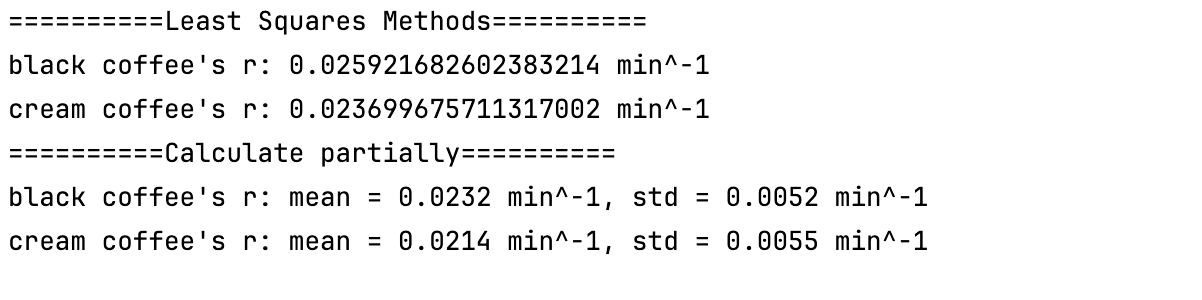
\includegraphics[width=\columnwidth]{1/a1.png}
\end{center}
\answer{b. 参见/1/b.py,图像中可见仍然存在一定的与实际值的误差。
		
		运行结果为	

		\begin{center}
			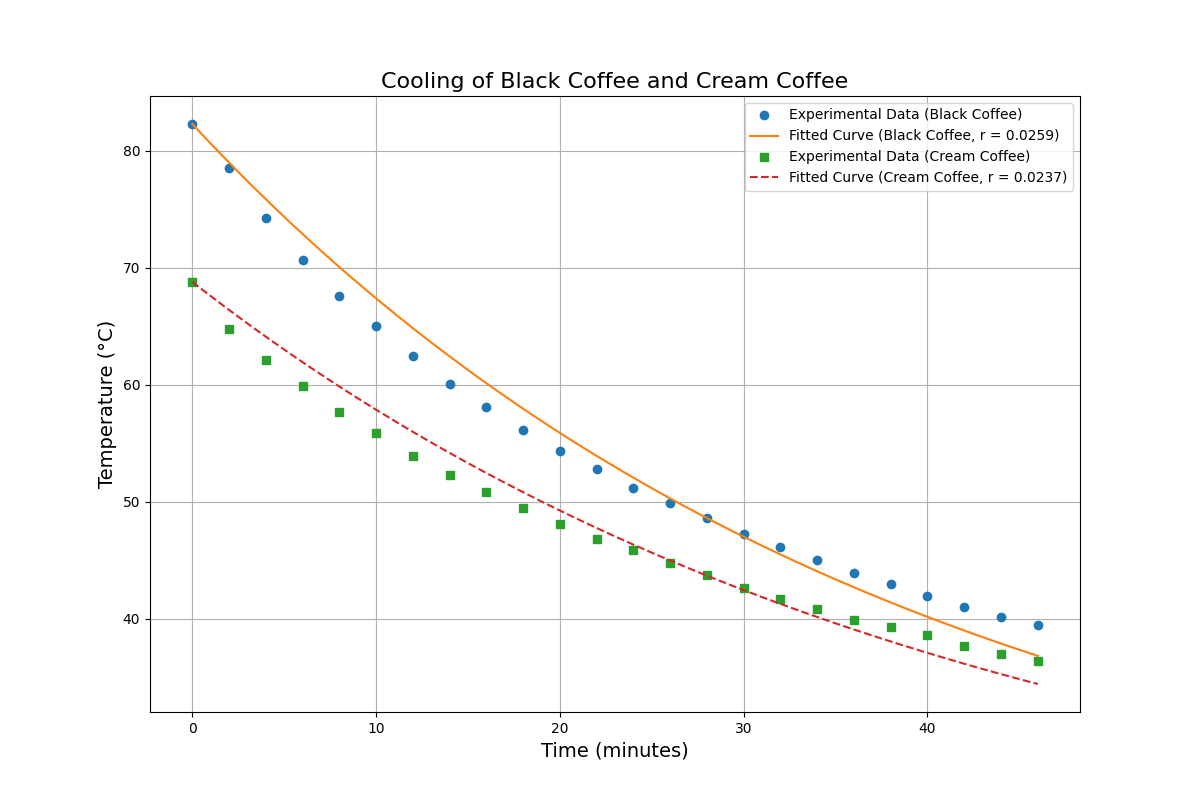
\includegraphics[width=0.7\columnwidth]{1/b.png}
		\end{center}}
\lstinputlisting[style = python]{1/b.py}
\answer{c. 设置两个新的步长4min和1min,其中4min步长通过直接取数据中的每个4min时间间隔即可,1min步长通过差值实现。}
\lstinputlisting[style = python]{1/c.py}
\answer{运行结果为}
\begin{center}
	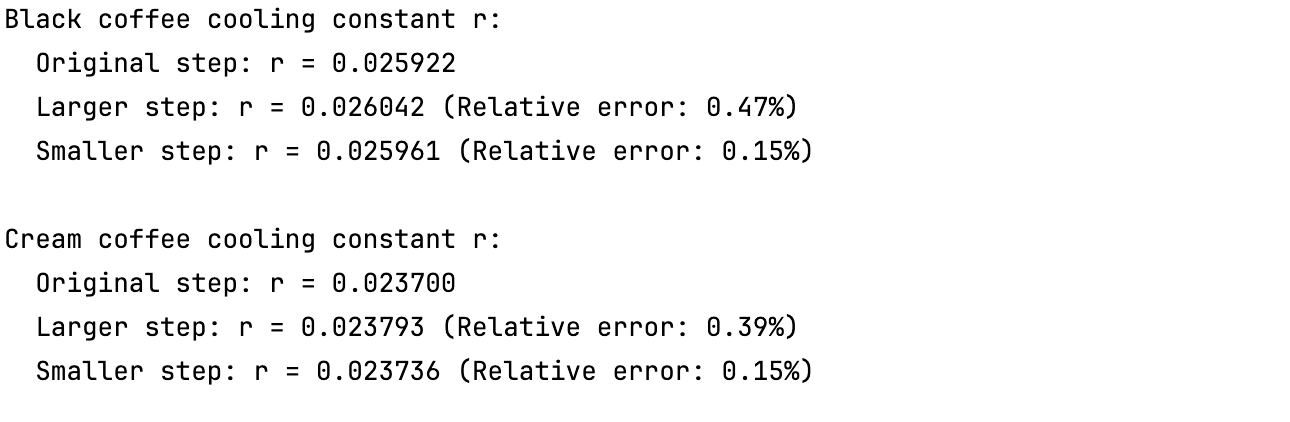
\includegraphics[width=\columnwidth]{1/c1.png}
\end{center}
\answer{d. 降温到49度需要27.54min,降温到33度需要54.30分钟,降温到25度需要81.06分钟。这说明物体与周围环境温差越小降温越慢。}
\lstinputlisting[style = python]{1/d.py}
\answer{运行结果为}
\begin{center}
	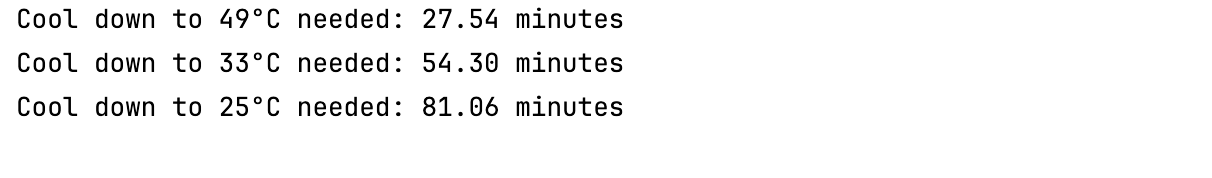
\includegraphics[width=\columnwidth]{1/d1.png}
\end{center}
\answer{e. 牛顿冷却定律并不完全适合这个问题,还存在液体的蒸发所带走的热量,以及液体表面积和与环境接触材质的影响,需要考虑物体与环境的热传导系数、物体的传热方式来进行优化。}
\end{question}

%----------------------------------------------------------------------------------------
%	QUESTION 2
%----------------------------------------------------------------------------------------

\begin{question}

\questiontext{Accuracy and stability of the Eular method.}

\answer{a. 牛顿冷却定律:$\frac{dT}{dt}=-r\times (T-T_{env})$,
		将T项移到左边后对时间从0到t积分得:$T(t)-T_{env}=e^{-rt}\times (T_0-T_{env})$,其中$T_0=T(\inf)=T_s$,可得$T(t)=T_s-(T_s-T_0)e^{-rt}$}

\lstinputlisting[style = python]{2/b.py}
\answer{运行结果为:

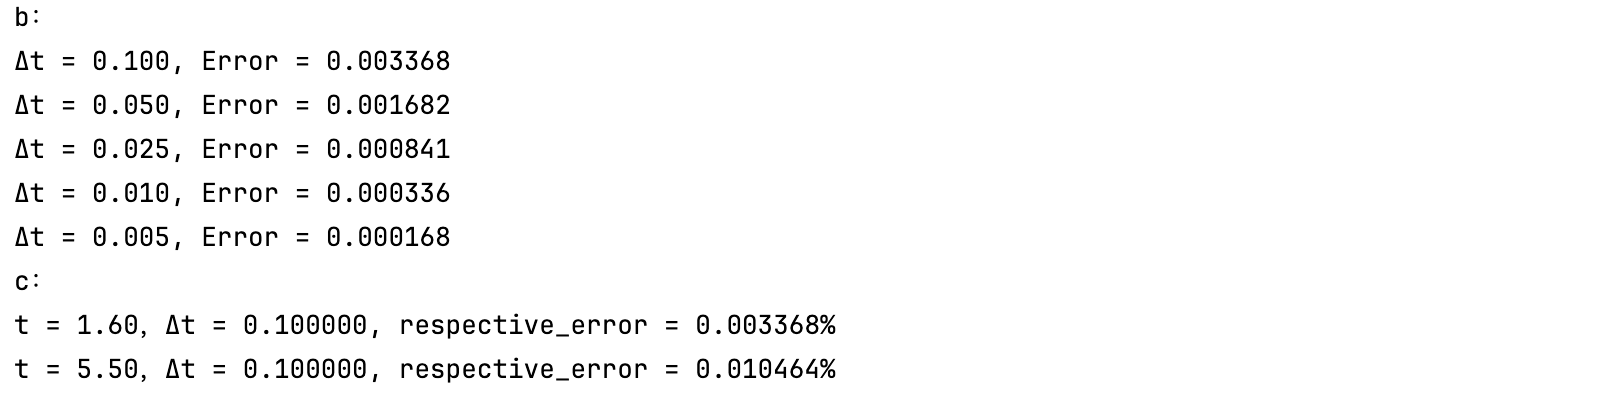
\includegraphics[width=\columnwidth]{2/b1.png}

		整理如下}

\begin{table}[h]
	\centering
	\begin{tabular}{l l}
		\toprule
		$\Delta t$& Error\\
		\midrule
		0.100&0.003368\\
		0.050&0.001682\\
		0.025&0.000841\\
		0.010&0.000336\\
		0.005&0.000168\\
		\bottomrule
	\end{tabular}
\end{table}
\begin{center}
	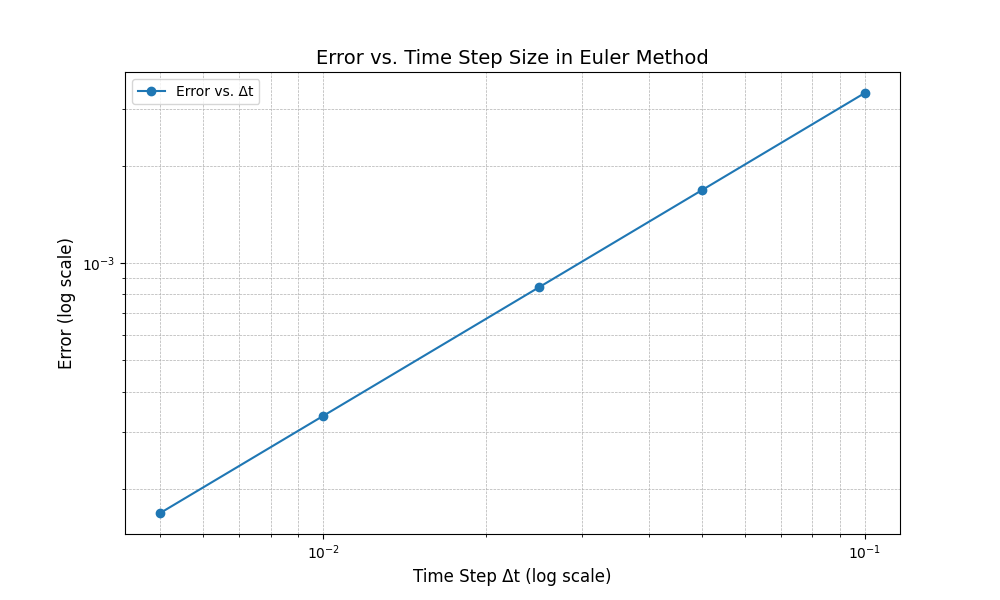
\includegraphics[width=0.7\columnwidth]{1/2_b.png}
\end{center}
\answer{由图可见,Eular method是1阶方法}
\answer{c. 由运行结果,$\Delta t=0.1$和$\Delta t=0.1$}

%--------------------------------------------
%--------------------------------------------

\end{question}
\iffalse
\begin{question}
	\questiontext{Comparison of algorithm.}
	\answer{a. 设置多个$\Delta t$:0.2s, 0.1s, 0.05s, 0.01s, 0.005s, 0.001s, 0.0005s, 0.0001s,分别计算相对误差并画表得}

	\begin{table}[h!]
		\centering
		\begin{tabularx}{\textwidth}{|X|X|X|X|X|X|X|}
		\hline
		$\Delta t$ & Euler (y error) & Euler (v error) & Euler-Cromer (y error) & Euler-Cromer (v error) & Euler-Richardson (y error) & Euler-Richardson (v error) \\
		\hline
		0.2    & 0.0780 & $3.625 \times 10^{-16}$ & 0.0780 & $3.625 \times 10^{-16}$ & $1.413 \times 10^{-16}$ & $3.625 \times 10^{-16}$ \\
		0.1    & 0.0387 & $3.625 \times 10^{-16}$ & 0.0387 & $3.625 \times 10^{-16}$ & $1.404 \times 10^{-16}$ & $3.625 \times 10^{-16}$ \\
		0.05   & 0.0193 & $7.250 \times 10^{-16}$ & 0.0193 & $7.250 \times 10^{-16}$ & $4.199 \times 10^{-16}$ & $7.250 \times 10^{-16}$ \\
		0.01   & 0.0039 & $5.257 \times 10^{-15}$ & 0.0039 & $5.257 \times 10^{-15}$ & $1.536 \times 10^{-15}$ & $5.257 \times 10^{-15}$ \\
		0.005  & 0.0019 & $9.788 \times 10^{-15}$ & 0.0019 & $9.788 \times 10^{-15}$ & $2.093 \times 10^{-15}$ & $9.788 \times 10^{-15}$ \\
		0.001  & 0.0004 & $2.936 \times 10^{-14}$ & 0.0004 & $2.936 \times 10^{-14}$ & $6.836 \times 10^{-15}$ & $2.936 \times 10^{-14}$ \\
		0.0005 & 0.0002 & $1.703 \times 10^{-13}$ & 0.0002 & $1.703 \times 10^{-13}$ & $3.391 \times 10^{-14}$ & $1.703 \times 10^{-13}$ \\
		0.0001 & 0.0000 & $2.976 \times 10^{-13}$ & 0.0000 & $2.976 \times 10^{-13}$ & $9.082 \times 10^{-14}$ & $2.976 \times 10^{-13}$ \\
		\hline
		\end{tabularx}
		\caption{Error values for different methods and $\Delta t$}
		\label{tab:error_values}
		\end{table}
\end{question}
\fi
\begin{question}
	\questiontext{Motion of a linear oscillator.}
	\answer{a. 参见/5/a.py}
	\lstinputlisting[style=python]{5/a.py}
	\begin{center}
		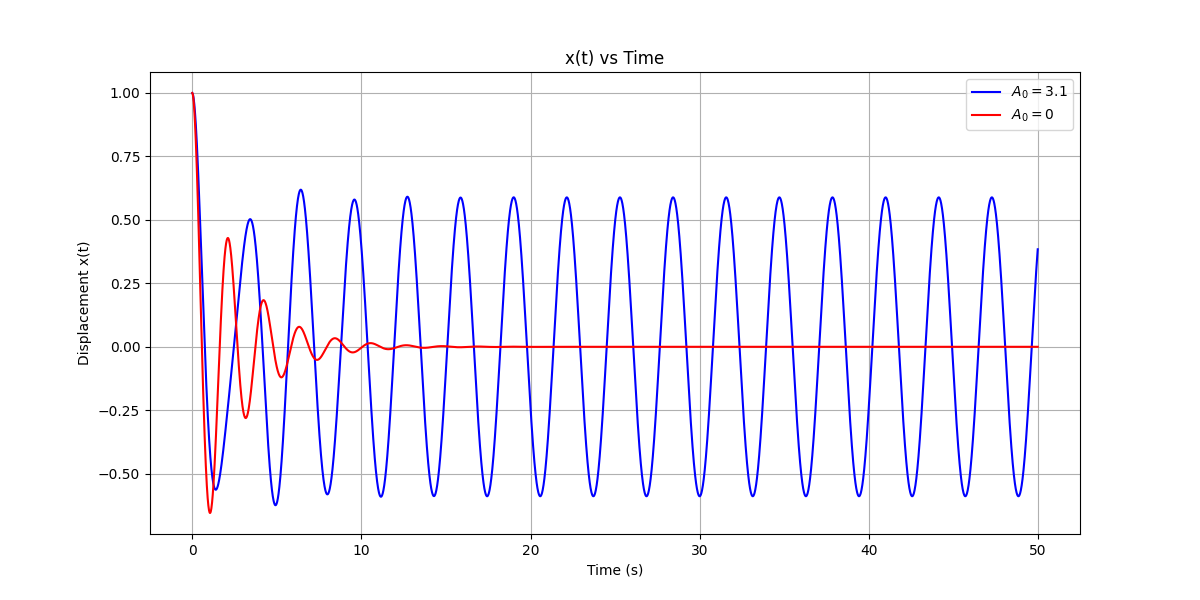
\includegraphics[width=\columnwidth]{5/a1.png}
	\end{center}

	\answer{Q1: 当 $A_0 = 3.1$ 时,与未受驱动力影响的情况 ($A_0 = 0$) 相比,位移 $x(t)$ 的行为发生了显著变化。首先,在 $A_0 = 0$ 的情况下,系统的运动表现为单调衰减至零的阻尼行为,即在初始位移之后,系统因阻尼逐渐失去能量,位移 $x(t)$ 以指数形式衰减,不会出现持续的周期性振荡。

	然而,当驱动力 $A_0 = 3.1$ 被引入后,系统的运动从单纯的阻尼衰减变为受驱动的强迫振荡。在初始阶段,系统的运动仍然包含一些瞬态行为,与 $A_0 = 0$ 的情况相似。然而,随着时间推移,这种瞬态行为逐渐消失,系统过渡到稳态振荡。在稳态阶段,系统以驱动力的频率 $\omega$ 振荡,而非系统的自然频率 $\omega_0$。驱动力的振幅 $A_0$ 决定了稳态振荡的振幅 $A(\omega)$,且其大小依赖于驱动力的频率 $\omega$ 和系统的自然频率 $\omega_0$ 之间的关系。
	
	此外,当驱动力的频率 $\omega$ 接近系统的自然频率 $\omega_0$ 时,共振效应显现,导致系统振幅显著增大。
	
	Q2: 计数估计$T=3.33s, \omega=1.88rad\cdot s^{-1}$,接近外驱动力频率。}
	\answer{b. 同为a.py的输出结果,见下图
	\begin{center}
		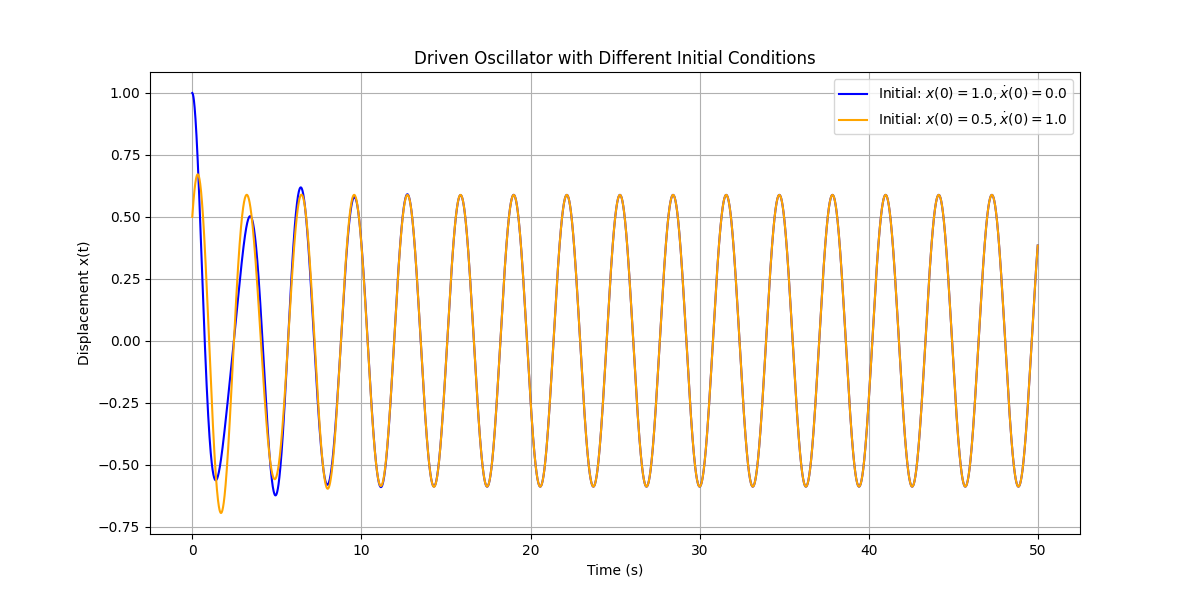
\includegraphics[width=\columnwidth]{5/b1.png}
	\end{center}

	Q3: 是的,在初始时刻,两振子由于不同初始条件有着明显不同的运动状态。在足够长时间后,在外驱动力的影响下,两种初始条件的振子都会达到与外驱动力相同的运动状态。
	}
	\answer{c. 参见/5/c.py}
	\lstinputlisting[style=python]{5/c.py}
	\answer{Q4: 能量不守恒,由于存在阻尼和外力,所以只有在外力提供被阻尼损耗掉的能量的情况下才能保持简谐振动,而振子本身能量是不守恒且随着周期性外力做周期性变化的。
	
	\begin{center}
		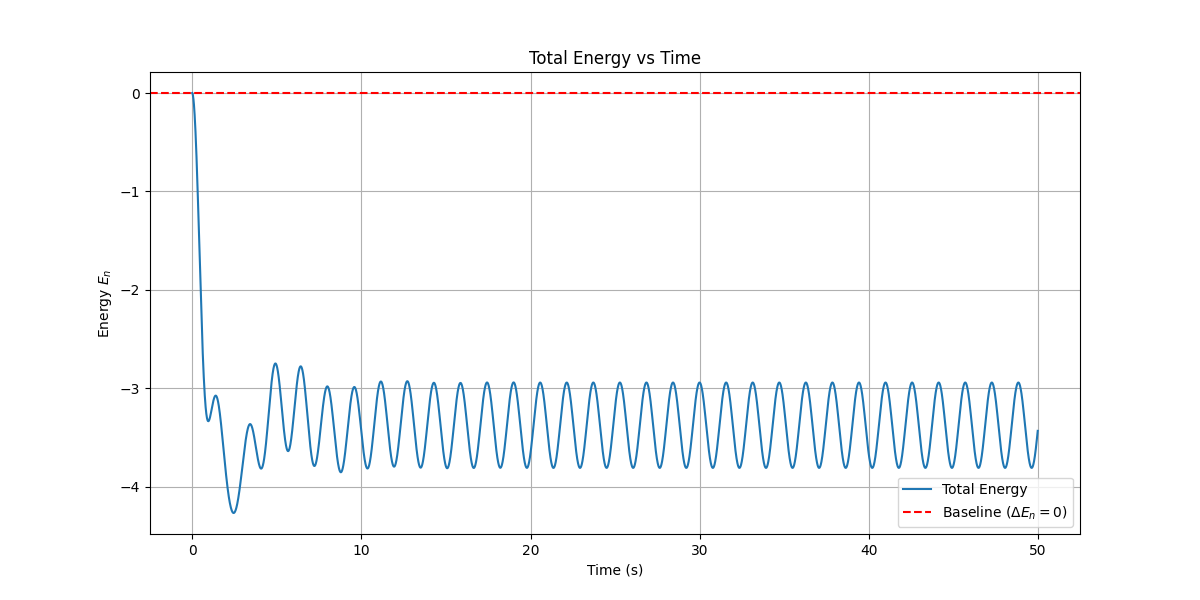
\includegraphics[width=\columnwidth]{5/c1.png}
	\end{center}}
	\answer{Q5: 
	\begin{center}
		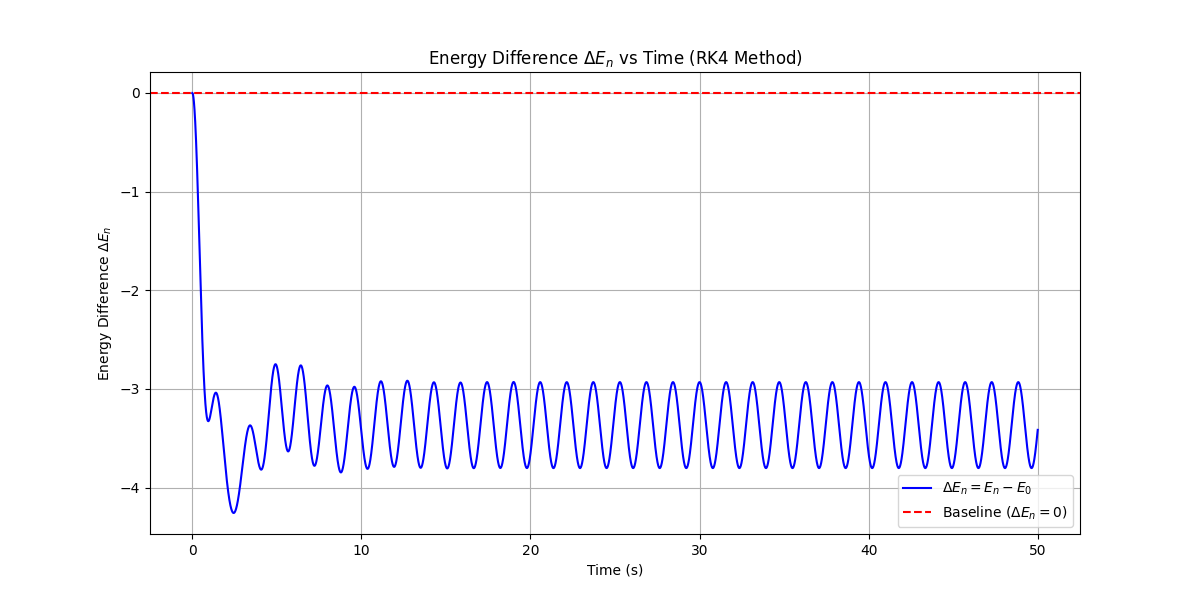
\includegraphics[width=\columnwidth]{5/c2.png}
	\end{center}
	}

	\answer{d. 参见/5/d.py}
	\lstinputlisting[style=python]{5/d.py}
	\answer{运行结果为:
	\begin{center}
		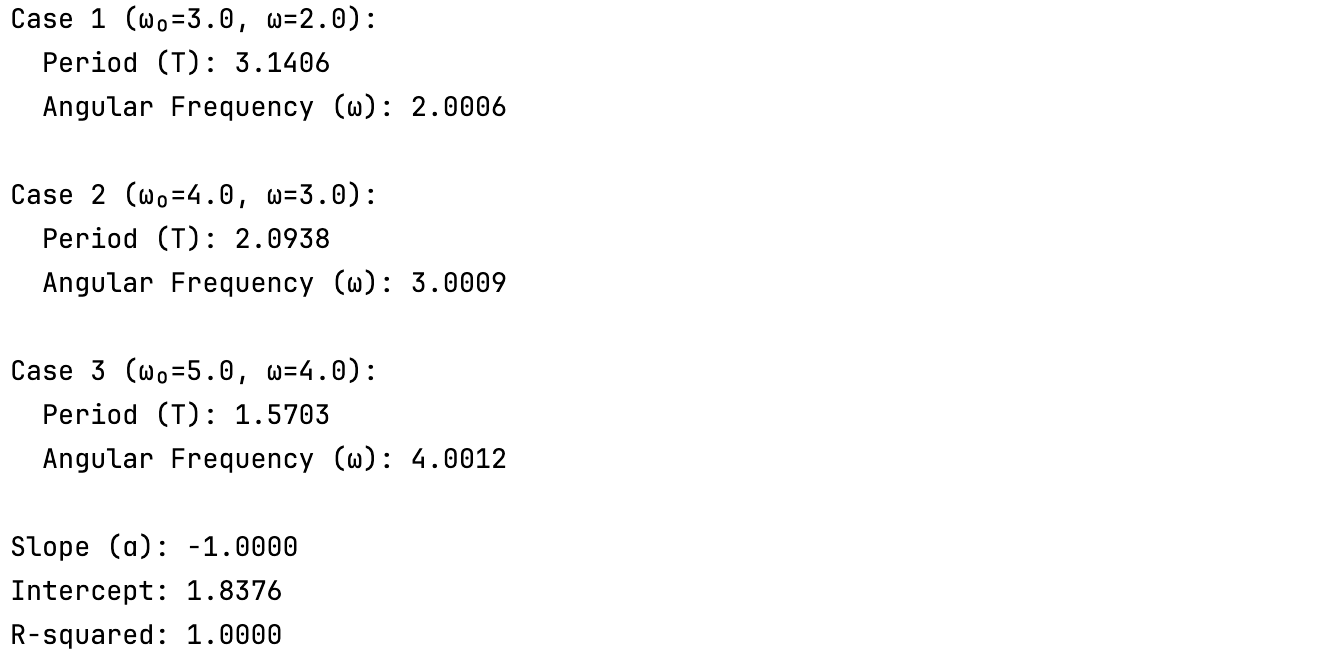
\includegraphics[width=\columnwidth]{5/d3.png}
	\end{center}
	\begin{center}
		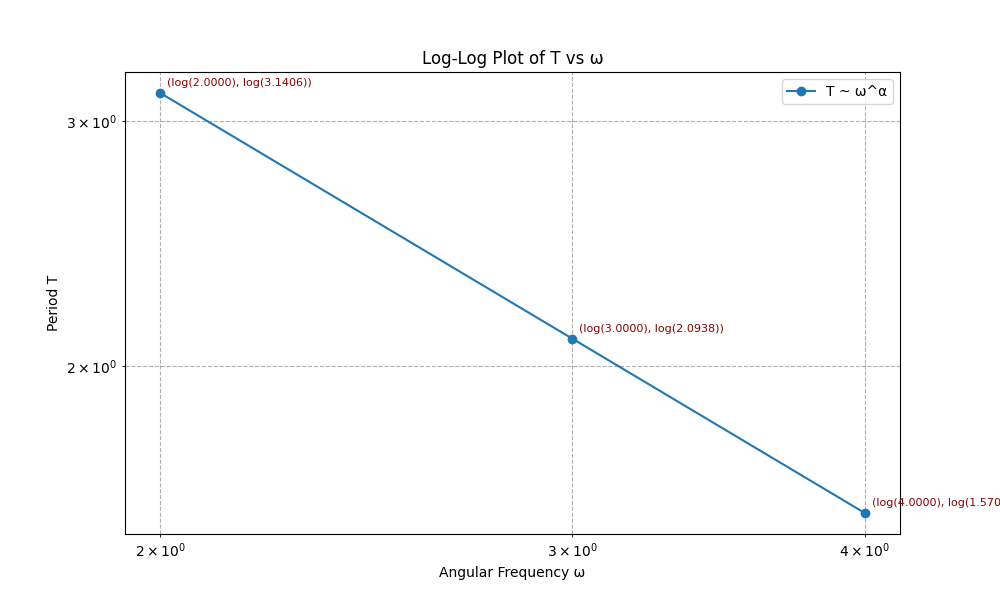
\includegraphics[width=\columnwidth]{5/d1.png}
	\end{center}
	直观上看log-log图像为直线,通过图中数据点线性拟合可得$\alpha=-1$,且由输出结果可以看到拟合的$R^2=1$,这说明拟合非常吻合。}
	\answer{Q6: 整理输出结果得}

	\begin{table}[h!]
		\centering
		\begin{tabular}{ccccc}
		\toprule
		\textbf{Case} & \(\boldsymbol{\omega_0}\) & \(\boldsymbol{\omega}\) & \textbf{Period (T)} & \textbf{Angular Frequency (\(\omega\))} \\
		\midrule
		Case 1 & 3.0 & 2.0 & 3.1406 & 2.0006 \\
		Case 2 & 4.0 & 3.0 & 2.0938 & 3.0009 \\
		Case 3 & 5.0 & 4.0 & 1.5703 & 4.0012 \\
		\bottomrule
		\end{tabular}
		\label{tab:oscillator_results}
		\end{table}
	\answer{Q7: 影响稳态时频率的因素是外驱动力频率,一定时间后振子会与外驱动力达到同频。由输出结果可得$\alpha=-1$和log-log图像}
	\answer{e. 参见/5/e.py}
	\lstinputlisting[style=python]{5/e.py}
	\begin{center}
		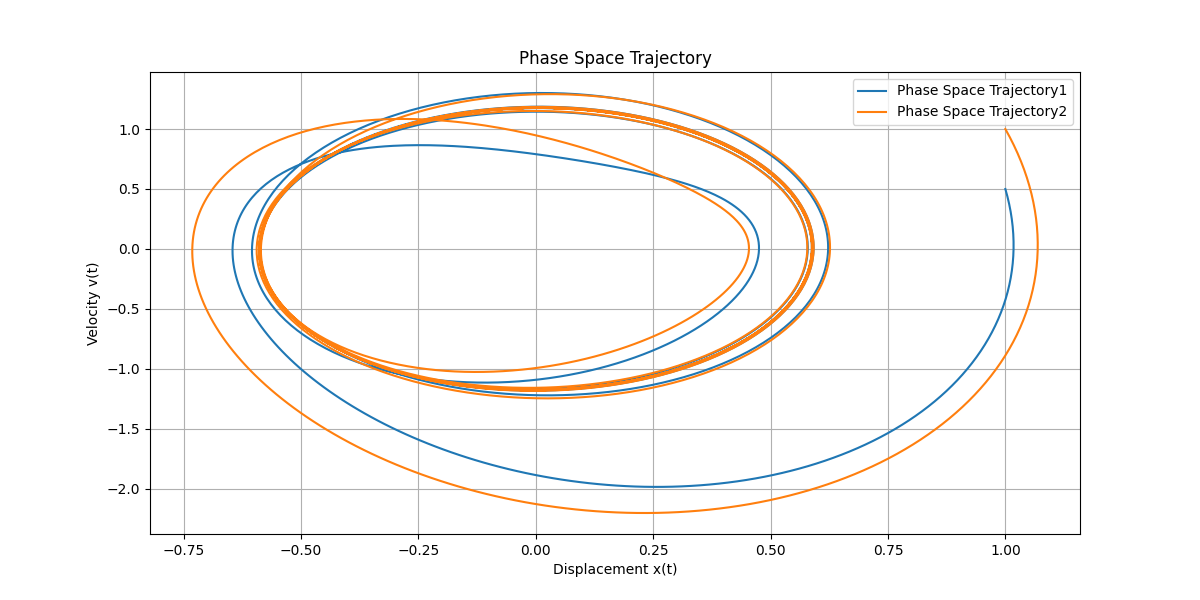
\includegraphics[width=\columnwidth]{5/e1.png}
	\end{center}
	
	\answer{图中trajctort1是初始条件x=1.0,v=0.5;trajctory2是x=1.0,v=1.0。可见两条图线在起始点和起始之后的一段距离上相空间图像不一样,在振子与外驱动力同频后便都在相同的位置进行周期性的运动,相空间图像表现为两个重合的椭圆。由图像可以看出两种振子由初始逐渐达到与外驱动力共振德过程。}
	\answer{f. 参见/5/f.py}
	\lstinputlisting[style=python]{5/f1.py}
	\answer{首先验证稳态的振子坐标的数值解可以表示成解析解:$x(t)=A(\omega)\cos(\omega t+\delta(\omega))$。在三组$\omega$下进行对稳态时数值解和解析解的绘图,可以看到两种图线十分重合,这说明稳态时振子的数值解可以表示成上述形式。
	
	代码输出结果如下}
	
	\begin{figure}[H]
		\centering
		% First image
		\begin{subfigure}{\textwidth}
			\centering
			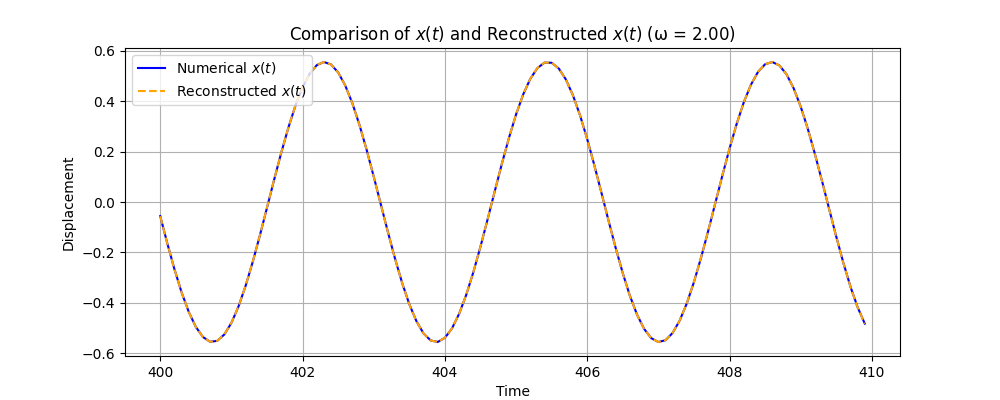
\includegraphics[width=\textwidth]{5/f1.png}
			%\caption{Image 1}
			\label{fig:f1}
		\end{subfigure}
		% Second image
		\begin{subfigure}{\textwidth}
			\centering
			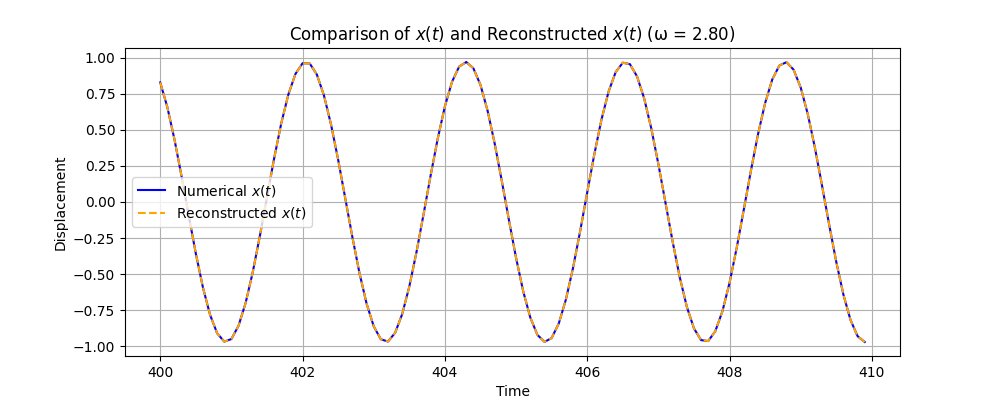
\includegraphics[width=\textwidth]{5/f2.png}
			%\caption{Image 2}
			\label{fig:f2}
		\end{subfigure}
		% Third image
		\begin{subfigure}{\textwidth}
			\centering
			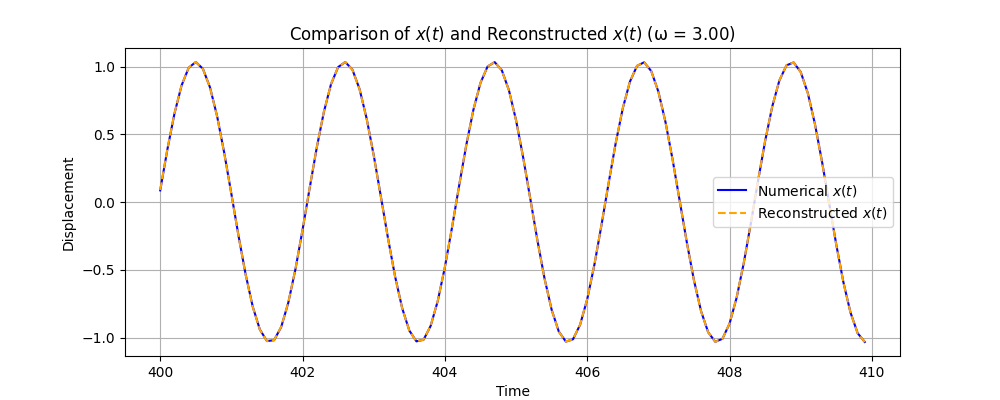
\includegraphics[width=\textwidth]{5/f3.png}
			%\caption{Image 3}
			\label{fig:f3}
		\end{subfigure}
	\end{figure}
	
	\begin{center}
		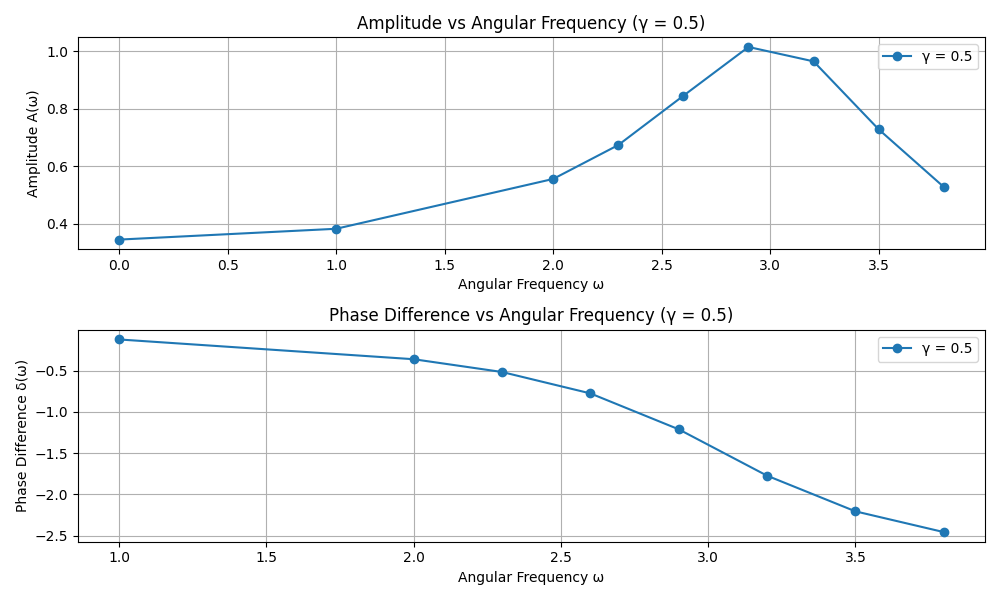
\includegraphics[width=\textwidth]{5/f4.png}
	\end{center}
	\begin{center}
		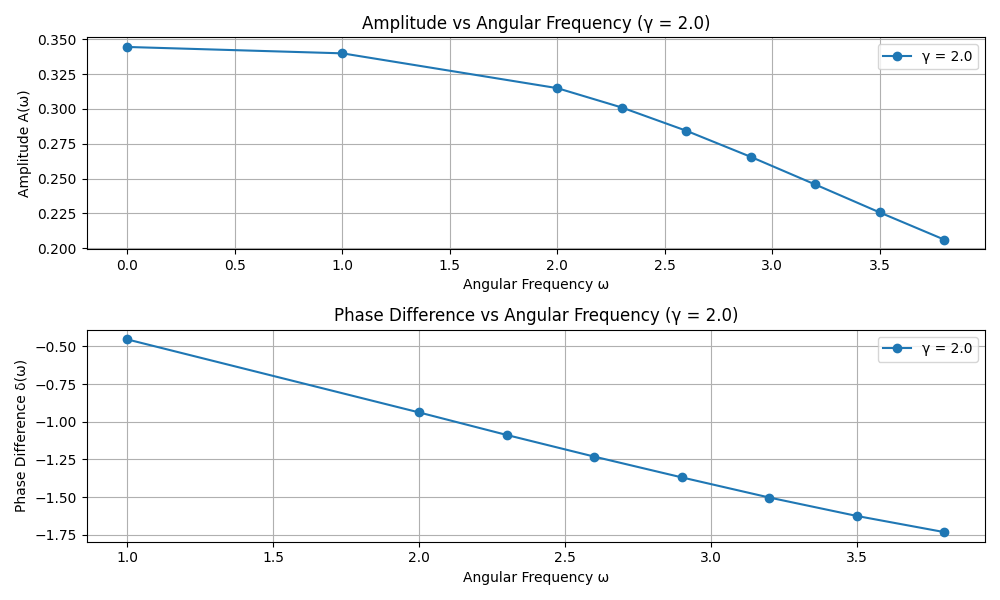
\includegraphics[width=\textwidth]{5/f5.png}
	\end{center}

	\begin{center}
		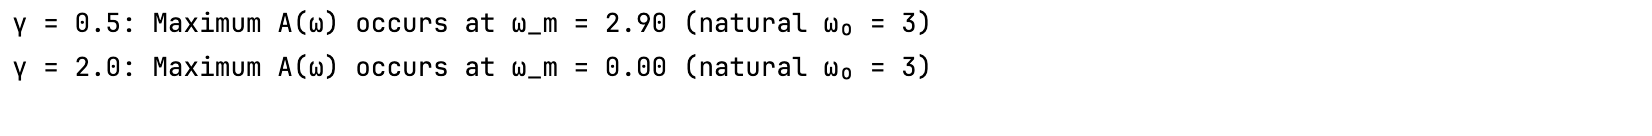
\includegraphics[width=\textwidth]{5/f6.png}
	\end{center}

	\answer{Q9: 见输出结果中的Amplitude vs Angular Frequency图和Phase Difference vs Angular Frequency图。}
	\answer{Q10: 见输出结果中的最后一张图,当阻尼系数为0.5时,存在最大振幅出现在$\omega=2.90$处,接近外驱动力频率。当阻尼系数为2.0时,相对来说阻尼系数较大,外驱动力不能抵抗阻尼力,所以表现出图像所示结果,即外驱动力角频率为0时振幅最大,而其他任意频率的外驱动力都不能抵消阻尼力,因此不能达到共振,导致振幅减小。
	
	与无外力的阻尼振子对比,无外力的阻尼振子在最开始时的频率是与自然频率$\omega_0$接近的,因此也与$\omega_m$很接近,而随着阻尼耗散,频率会指数形降低最后静止。}

	
\end{question}
%----------------------------------------------------------------------------------------
%	QUESTION 3
%----------------------------------------------------------------------------------------
\iffalse
\begin{question}

\questiontext{Identify the author of Equation \ref{eq:bayes} below and briefly describe it in English.}

\begin{equation}\label{eq:bayes}
	P(A|B) = \frac{P(B|A)P(A)}{P(B)}
\end{equation}

\answer{Lorem ipsum dolor sit amet, consectetur adipiscing elit. Praesent porttitor arcu luctus, imperdiet urna iaculis, mattis eros. Pellentesque iaculis odio vel nisl ullamcorper, nec faucibus ipsum molestie. Sed dictum nisl non aliquet porttitor. Etiam vulputate arcu dignissim, finibus sem et, viverra nisl. Aenean luctus congue massa, ut laoreet metus ornare in. Nunc fermentum nisi imperdiet lectus tincidunt vestibulum at ac elit. Nulla mattis nisl eu malesuada suscipit.}

\end{question}

%----------------------------------------------------------------------------------------

\assignmentSection{Bonus Questions}

%----------------------------------------------------------------------------------------
%	QUESTION 4
%----------------------------------------------------------------------------------------

\begin{question}

\questiontext{The table below shows the nutritional consistencies of two sausage types. Explain their relative differences given what you know about daily adult nutritional recommendations.}

\begin{table}[h]
	\centering % Centre the table
	\begin{tabular}{l l l}
		\toprule
		\textit{Per 50g} & Pork & Soy \\
		\midrule
		Energy & 760kJ & 538kJ\\
		Protein & 7.0g & 9.3g\\
		Carbohydrate & 0.0g & 4.9g\\
		Fat & 16.8g & 9.1g\\
		Sodium & 0.4g & 0.4g\\
		Fibre & 0.0g & 1.4g\\
		\bottomrule
	\end{tabular}
\end{table}

\answer{Lorem ipsum dolor sit amet, consectetur adipiscing elit. Praesent porttitor arcu luctus, imperdiet urna iaculis, mattis eros. Pellentesque iaculis odio vel nisl ullamcorper, nec faucibus ipsum molestie. Sed dictum nisl non aliquet porttitor. Etiam vulputate arcu dignissim, finibus sem et, viverra nisl. Aenean luctus congue massa, ut laoreet metus ornare in. Nunc fermentum nisi imperdiet lectus tincidunt vestibulum at ac elit. Nulla mattis nisl eu malesuada suscipit.}

\end{question}

%----------------------------------------------------------------------------------------
%	QUESTION 5
%----------------------------------------------------------------------------------------

\begin{question}

\lstinputlisting[style = python]{5/a.py}


%--------------------------------------------

\begin{subquestion}{How many luftballons will be output by the Listing \ref{lst:luftballons} above?} % Subquestion within question

\answer{99 luftballons.}

\end{subquestion}

%--------------------------------------------

\begin{subquestion}{Identify the regular expression in Listing \ref{lst:luftballons} and explain how it relates to the anti-war sentiments found in the rest of the script.} % Subquestion within question

\answer{Lorem ipsum dolor sit amet, consectetur adipiscing elit. Praesent porttitor arcu luctus, imperdiet urna iaculis, mattis eros. Pellentesque iaculis odio vel nisl ullamcorper, nec faucibus ipsum molestie. Sed dictum nisl non aliquet porttitor. Etiam vulputate arcu dignissim, finibus sem et, viverra nisl. Aenean luctus congue massa, ut laoreet metus ornare in. Nunc fermentum nisi imperdiet lectus tincidunt vestibulum at ac elit. Nulla mattis nisl eu malesuada suscipit.}

\end{subquestion}

%--------------------------------------------

\end{question}
\fi
%----------------------------------------------------------------------------------------

\end{document}
